\documentclass[12pt,fleqn,twoside]{book}
\title{Shr\"odinger's Wave Function}
\author{Himalaya Satyal\footnote{Rato Bangala School}}
\usepackage{pgfplots}
\usepackage{layout}
\usepackage{cancel}
\usepackage{amsmath}
\usepackage{flushend}
\usepackage[a5paper, margin=1in]{geometry}
\usepackage{amssymb}
\usepackage{ragged2e}
\usepackage{esdiff}
\pgfplotsset{compat=1.18}
\begin{document}
\maketitle 
\[
    \int_a^bf(x)\mathrm{d}x=\int_0^bf(x)\mathrm{d}x-\int_0^af(x)\mathrm{d}x
\]
Hello I am Himalaya Satyal and this is a research on Shr\"odinger's wave equations.The Shr\"odinger Equation is $i\hbar \frac{\partial}{\partial t}|\Psi\rangle = \hat{H}|\Psi\rangle$ By 
definition,$\int_a^bf(x)\mathrm{d}x=\int_0^bf(x)\mathrm{d}x-\int_0^af(x)\mathrm{d}x$. 
\[
E_k+E_P=E_T\]\[\Longrightarrow \frac{-\hbar^2}{2m}\nabla^2\Psi(r)+V(r)\Psi(r)=E\Psi(r)\]
\[ x\equiv -1 \pmod{5}\]\[i\hbar \frac{\partial}{\partial t}|\Psi\rangle = \hat{H}|\Psi\rangle\]
\[\Longrightarrow x+1\equiv0\pmod{5}\]
\centering Therefore, $5|x+1$
\RaggedRight Let $m$ be a fixed integer greater than 1. The sequence $x_0,x_1,x_2,\ldots$ is defined as follows:\\
\[x_i=\begin{cases}2^i&\text{if}\, 0\le j \le m-1; \\ \sum_{j=1}^m{x_{i-j}}&\text{if} \,i \ge m\end{cases}\]
Find the greatest $k$ for which the sequence contains 
$k$  consecutive terms \\ divisible by $m$.
\\ If $p$ is a prime and $p\nmid a$, then $a^p\equiv a \pmod{p}$ This is known as Fermat's Last Theorem.      \\A modified version of the Fermat's Last Theorem which gives: \\$a^{\phi(n)}\equiv1\pmod{n}$ where $\phi(n)$ is the Euler's Totient Function.
\newpage

Find the greatest $k$ for which the sequence contains 
$k$  consecutive terms \\ divisible by $m$.

    \[\oint_{e^{-i\pi}}^{\infty}\sin x\,\,\mathrm{d} x=?\]
    \[x=x_0\cos (\omega t)\]
\begin{equation}\Longrightarrow\diff{x}{t}=-\omega x_0 \sin (\omega t)\end{equation}
    \[v=v_0\sin (\omega t)\]
    \begin{equation}\Longrightarrow \diff{v}{t}=-\omega ^2 x_0 \cos (\omega t)\end{equation}
    \[a=a_0\cos (\omega t)\]
    \[a_0=-\omega^2 x_0\]
    \[x=x_0 e^{-\lambda t}\]
    \[\Longrightarrow \diff{x}{t}=-\lambda x_0 e^{-\lambda t}\]
\newpage
\[\frac{\partial x}{\partial t}=\partial \vec{A}\]
\begin{equation}
pV=\frac 1 3 Nm{\langle c^2\rangle}
\end{equation}
\[\Longrightarrow c_{r.m.s}=\sqrt{\langle c^2\rangle}\]
Now we will look at the workfunction relation between the energy of photon and maximum kinetic energy of a photoelectron emitted.
\[E_{photon}=hf=\varPhi+E_{k-max} \]
\begin{equation}\therefore E_k=hf-\varPhi \end{equation}
Also $E_k=\frac 1 2 mv^2$, so:
\[\frac 1 2 m{v_{max}}^2=hf-\varPhi\]
\[hf=\varPhi+\cancelto{0}{E_{k}} \]
\[\mathrm{From\;eq^n (4):}\;hf_0=\varPhi\]
\newpage
\section{Maxwell's Equations}
\title{Differential Form}
\[\nabla \cdot \mathbf{E}=\frac {\rho}{{\varepsilon}_0}\]
\[\nabla \cdot \mathbf{B}=0\]
\[\nabla \times \mathbf{E}=-\frac{\partial \mathbf{B}}{\partial t}\]
\[\nabla \times \mathbf{B}={\mu}_0\bigg(\mathbf{J}+\varepsilon_0\frac{\partial \mathbf{E}}{\partial t}\bigg)\]
\raggedright
\title{Integral Form}
\[\oint_S\vec{E}\cdot\mathrm{d} \vec{a}=\frac{Q_{enc}}{\varepsilon_0}\]
\[\oint_S\vec{B}\cdot\mathrm{d}\vec{a}=0\]
\[\oint_C\vec{E}\cdot\mathrm{d}\vec{l}=\int_{S}\frac{\partial \vec{B}}{\partial t}\cdot \mathrm{d} \vec{a}\]
\[\oint_C\vec{B}\cdot\mathrm{d}\vec{l}=\mu_0\mathit{I}+\mu_0\varepsilon_0\int_{S}\frac{\partial \vec{E}}{\partial t}\cdot \mathrm{d} \vec{a}\]
\newpage
Now, let's take a look at the activity and half-life of a radioactive substance.
\[-\frac{\mathrm{d}N}{\mathrm{d}t}\propto N\]
\[\Longrightarrow\frac{\mathrm{d}N}{\mathrm{d}t}=-\lambda N\]
\[\Longrightarrow\frac{1}{N}\;\mathrm{d}N=-\lambda\;\mathrm{d}t\]
Integrate both sides: 
\[\int_{N_0}^{N}\frac 1 N\;\mathrm{d}N=-\lambda\int_{0}^{t}1\;\mathrm d t\;\;\;\;\big[\because N=N_0 \textrm{ at } t=0\;\big]\]
\[\Longrightarrow \Big[\;\mathrm{\ln}N\;\Big]^{N}_{N_0}=-\lambda\Big[\;t\;\Big]_0^t\]
\[\Longrightarrow \mathrm{ln}N-\mathrm{ln}N_0=-\lambda t\]
\[\Longrightarrow \mathrm{ln}\bigg(\frac{N}{N_0}\bigg)=-\lambda t\]
\[\Longrightarrow\frac{N}{N_0}=\mathrm{e}^{-\lambda t}\]
\[\therefore N=N_0\;\mathrm{e}^{-\lambda t}\]
\[\Longrightarrow \lambda=\frac{\mathrm{ln}2}{t_\frac{1}{2}}\]
\[\therefore t_\frac{1}{2}=\frac{\mathrm{ln}2}{\lambda}\]
\[\therefore A=A_0\;\mathrm{e}^{-\lambda t}\;\;\;\big[\because A=N\lambda\big]\]
\[L=4\pi\sigma r^2T^4\]
\[F=\frac L {4\pi d^2}\]
\[\lambda_{\mathrm{max}}\propto\frac{1}{T}\]
\[f=f_0\frac{v}{v \pm v_\mathrm {s}}\]
\newpage
\section{Taylor Series}
\[x\equiv-1 \pmod 5\]
\[\frac{-\hbar^2}{2m}\nabla^2\Psi(r)+V(r)\Psi(r)=E\Psi(r)\]
\[i\hbar \frac {\partial}{\partial t}|\Psi\rangle=\hat{H}|\Psi\rangle\]
\[y=\begin{cases}2^i & 0\leqslant j\leqslant m-1;\\\sum_{j=1}^m x_{i-j}&i\geqslant m \end{cases}\]
\[\begin{bmatrix} 1&2\\3&4\end{bmatrix}\begin{bmatrix}2&7\\3&4\end{bmatrix}=\begin{bmatrix}8&15\\18&37\end{bmatrix}\]
\newpage
\section{The photoelectric effect}
\[\Phi=\mathrm{K.E.}_{max}+hf\]
\[\therefore E_{k(max)}=\Phi-hf\]
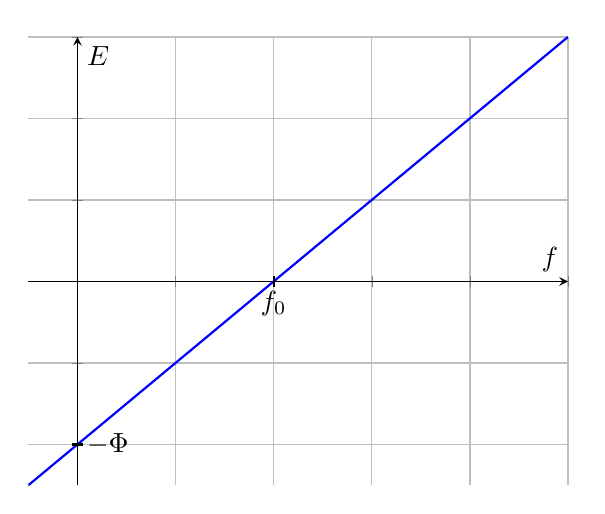
\begin{tikzpicture}
    \begin{axis}[
        axis lines=center,
        xlabel=$f$,
        ylabel=$E$,
        xmin=-1, xmax=10,
        ymin=-5,ymax=6,
        xticklabels=\empty,
        yticklabels=\empty,
        xtick distance=2,
        ytick distance=2,
        grid=both,
        grid style={line width=0.5pt},
    ];
    \addplot[domain=-10:10,blue, thick] {x-4};
    \addplot[mark=|,thick,color=black] coordinates {(4,0)};
    \addplot[mark=-,thick,color=black] coordinates {(0,-4)};
    \node at (axis cs:4,0) [anchor=north] {$f_0$};    
    \node at (axis cs:0,-4)[anchor=west]{$-\Phi$};
\end{axis}
\end{tikzpicture}
\[E=\begin{cases}0&\mathrm{at}\;0\leqslant f\leqslant f_0\\ hf-\Phi&\mathrm{at}\;f > f_0\end{cases}\]
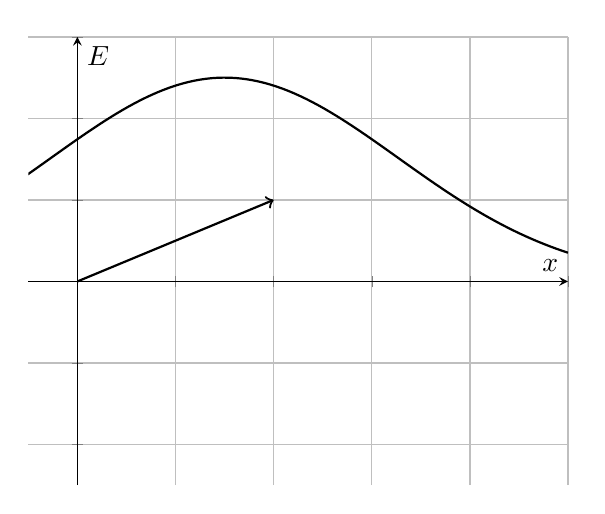
\begin{tikzpicture}
    \begin{axis}
        [
            axis lines=center,
            xlabel=$x$,
            ylabel=$E$,
            xmin=-1, xmax=10,
            ymin=-5,ymax=6,
            xticklabels=\empty,
            yticklabels=\empty,
            xtick distance=2,
            ytick distance=2,
            grid=both,
            grid style={line width=0.5pt},
        ];
    \addplot[samples=100, thick, domain=-2:10]{5*e^-((x-3)^2/25)};
    \addplot[->, thick, color=black]coordinates{(0,0) (4,2)};
\end{axis}
\end{tikzpicture}
\[E_{p}=m\Delta\varPhi\]
\[E_p=-m\bigg(\frac{GM}{{R_2}}-\frac{GM}{{R_1}}\bigg)\]
\[\therefore E_p=GMm\bigg(\frac{1} {{R_1}}-\frac{1} {{R_2}}\bigg)\]
$x-y=0$
\newpage
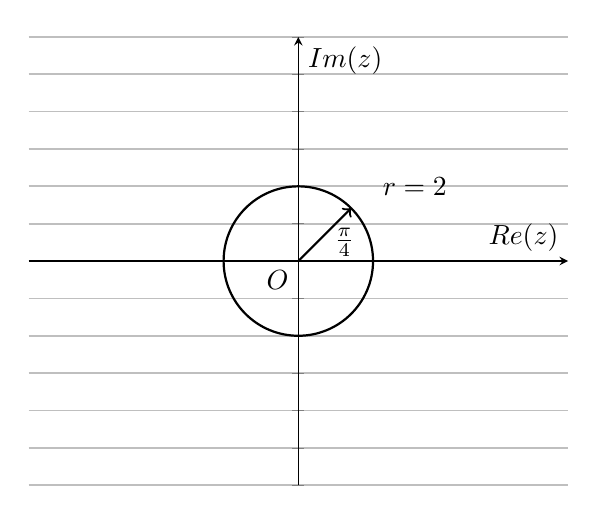
\begin{tikzpicture}
    \begin{axis}
    [
        axis lines=center,
        xlabel=$Re(z)$,
        ylabel=$Im(z)$,
        xmin=-3,xmax=3,ymin=-3,ymax=3,
        xtick distance=4, ytick distance=0.5,
        xticklabels=\empty,
        yticklabels=\empty,
        grid=both,
        grid style={line width=0.6pt},
        axis equal
    ];
    \node at (axis cs:0,0)[anchor=north east]{$O$};
    \draw [black,thick] (axis cs:0,0)circle[radius=1];
    \pgfmathsetmacro{\x}{1/(sqrt(2))}
    \addplot[->,thick, color=black]coordinates{(0,0)(\x,\x)};
    \node at (axis cs:1,1)[anchor=west]{$r=2$};
    \node at (axis cs:0.35,0.25)[anchor=west]{$\frac{\pi}{4}$};
\end{axis}
\end{tikzpicture}
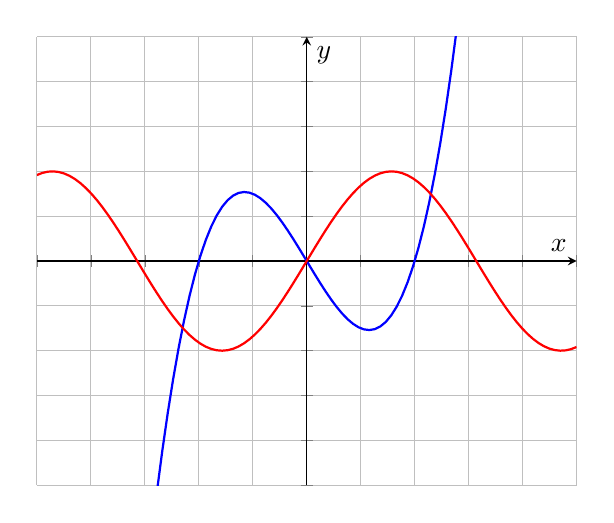
\begin{tikzpicture}
    \begin{axis}[
        axis lines=center,
        xlabel=$x$,
        ylabel=$y$,
        xtick distance=1,ytick distance=1,
        xticklabels=\empty,
        yticklabels=\empty,
        xmin=-5,xmax=5,
        ymin=-5,ymax=5,
        grid=both];
        \addplot[
            domain=-5:5,
            thick,
            samples=100,
            color=blue
        ]{(x-2)*(x+2)*x/2};
        \addplot[
            domain=-5:5,
            thick,
            samples=100,
            color=red
        ]{2*sin(deg(x))};
    \end{axis}
\end{tikzpicture}
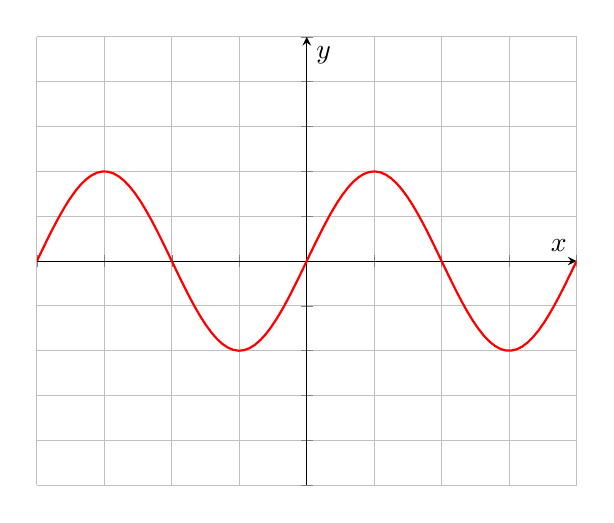
\begin{tikzpicture}
    \begin{axis}[
        axis lines=center,
        xlabel=$x$,
        ylabel=$y$,
        xtick distance=90,ytick distance=1,
        xticklabels=\empty,
        yticklabels=\empty ,
        xmin=-360,xmax=360,
        ymin=-5,ymax=5,
        grid=both];
        \addplot[
            domain=-360:360,
            thick,
            samples=100,
            color=red
        ]{2*sin(x)};
    \end{axis}
\end{tikzpicture}
\newline
\[\frac{2}{4}\oint^7_\pi 2x^2\; \mathrm{d}x\]
\begin{tikzpicture}
    \begin{axis}
        
    \end{axis}
\end{tikzpicture}
\end{document}
